\documentclass[11pt]{article}

\usepackage{fullpage}
\usepackage{rotating}   
\usepackage{amsmath}
\usepackage{amssymb}
\usepackage{amsthm}
\usepackage{fancyhdr}
\usepackage{algorithm}
\usepackage{algorithmic}
\usepackage{bm}
\usepackage{listings}
\usepackage{graphicx}
\usepackage{caption2}
\usepackage{subfigure}
\usepackage{float}
\usepackage{extpfeil}
\usepackage{color}
\usepackage[usenames,dvipsnames]{xcolor}


\newtheorem{theorem}{Theorem}[section]
\newtheorem{lemma}[theorem]{Lemma}
\newtheorem{corollary}[theorem]{Corollary}
\newtheorem{proposition}[theorem]{Proposition}
\newtheorem{definition}[theorem]{Definition}
\newtheorem{conjecture}[theorem]{Conjecture}
\newtheorem{remark}[subsection]{Remark}

%%
\newcommand\numberthis{\addtocounter{equation}{1}\tag{\theequation}}

%% define new symbols
\def\bx{\bm{x}}
\def\bb{\bm{b}}
\def\ba{\bm{a}}
\def\bc{\bm{c}}
\def\bf{\bm{f}}
\def\by{\bm{y}}
\def\bu{\bm{u}}
\def\bv{\bm{v}}
\def\BW{\bm{W}}
\def\BA{\bm{A}}
\def\bz{\bm{z}}
\def\BZ{\bm{Z}}
\def\BH{\bm{H}}
\def\BL{\bm{L}}
\def\BU{\bm{U}}
\def\BV{\bm{V}}
\def\BB{\bm{B}}
\def\BC{\bm{C}}
\def\BD{\bm{D}}
\def\BE{\bm{E}}
\def\BW{\bm{W}}
\def\BQ{\bm{Q}}
\def\BG{\bm{G}}
\def\BA{\bm{A}}
\def\BX{\bm{X}}
\def\BY{\bm{Y}}
\def\BQ{\bm{Q}}
\def\BI{\bm{I}}
\def\BR{\bm{R}}

%% define new brackets
\def\la{\left\langle}
\def\ra{\right\rangle}
\def\ln{\left\|}
\def\rn{\right\|}
\def\lb{\left(}
\def\rb{\right)}
\def\lsb{\left[}
\def\rsb{\right]}
\def\lcb{\left\{}
\def\rcb{\right\}}

%%
\DeclareMathOperator*{\argmin}{arg\,min}
\DeclareMathOperator*{\argmax}{arg\,max}

%%
\title{Homework XII}
\author{Name: Shao Yanjun, Number: 19307110036}


\begin{document}
\maketitle

%------------------------------------
\begin{abstract}
This is Daniel's homework of  "Numerical Algorithms with Case Studies II".
\end{abstract}
%-------------------------------------
%=====================
\section{Problems}
\paragraph{Q1}
Implement the code and examine the truncation error of RK4 on loglog() plots.
\begin{figure}[H]
	\centering
	\subfigure[truncation error]{
		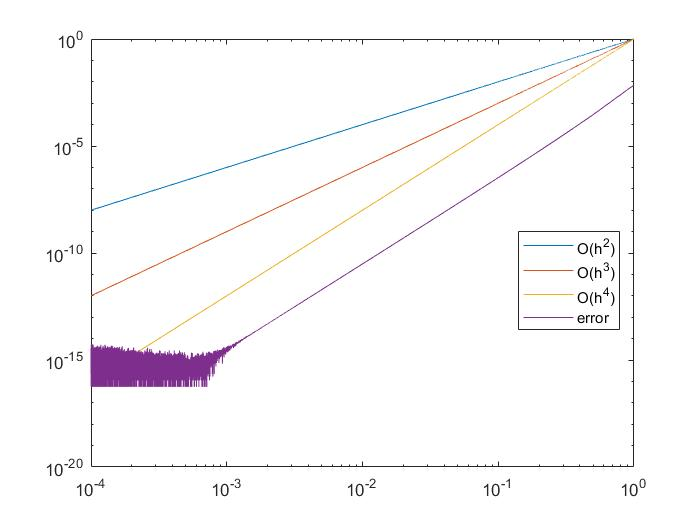
\includegraphics[width=0.8\linewidth]{error.jpg}
	}
\end{figure}
Most of the truncation error satisfy $O(h^4)$ level, while further accuracy cannot be reached because of rounding error.
\paragraph{Q2}
In this implicit method, we will have the following loop invariant in each iteration.
\begin{align}
	u_{k+1}&=u_k+h(\theta f(t_k+h,u_{k+1})+(1-\theta)f(t_k,u_k))\\
	&=u_k-h\theta\lambda u_{k+1}-h(1-\theta)\lambda u_k
\end{align}
So after each iteration, we will have,
\begin{align}
	u_{k+1}=\frac{1-h(1-\theta)\lambda}{1+h\theta\lambda}u_k
\end{align}
And to make $u_k\rightarrow0$ when $k\rightarrow\infty$, we have to let,
\begin{align}
	\frac{1-h(1-\theta)\lambda}{1+h\theta\lambda}<1
\end{align}
Which gives $h>0$.\\
However, this is not sufficient for convergence, because we must take a good step $h$ to make sure every implicit equation converges within each iteration. That gives the condition that $x=(1-h(1-\theta)\lambda)y-h\theta\lambda x$ must converge.
\begin{align}
	\|x_k+1-x_k\|&=h\theta\lambda\|x_k-x_{k-1}\|\\
	h&<\frac{1}{\theta\lambda}
\end{align} 
Therefore, $h\in (0,\dfrac{1}{\theta\lambda})$. However, numerical studies show that there could be an even tighter upper bound for stepsize.
\paragraph{Q3}
The stationary concentrations are approximately $X=0.097754, C=0.097749
,S=0.814495$
\begin{figure}[H]
	\centering
	\subfigure[solution]{
		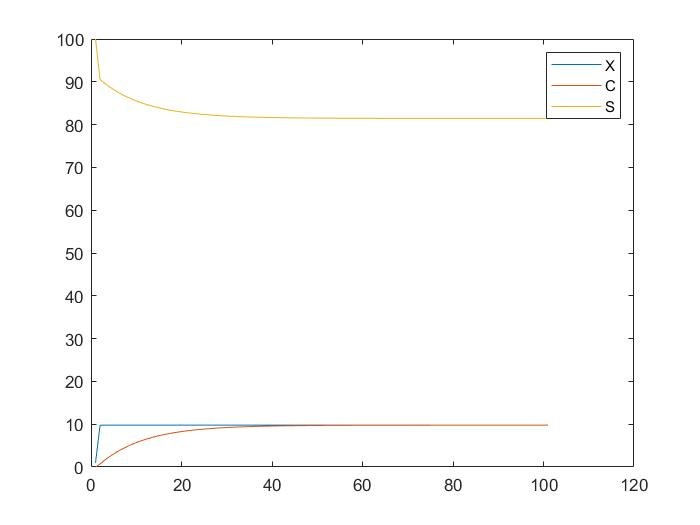
\includegraphics[width=0.8\linewidth]{res.jpg}
	}
\end{figure}
\paragraph{Q4}


%-------------------------------------
%=====================
\end{document}
